\section{Durchführung}
\label{sec:Durchführung}
\subsection{Aufbau}
Für diesen Versuch wird der in \autoref{fig:Versuchsaufbau} verwendete Aufbau genutzt.
\begin{figure}
    \centering
    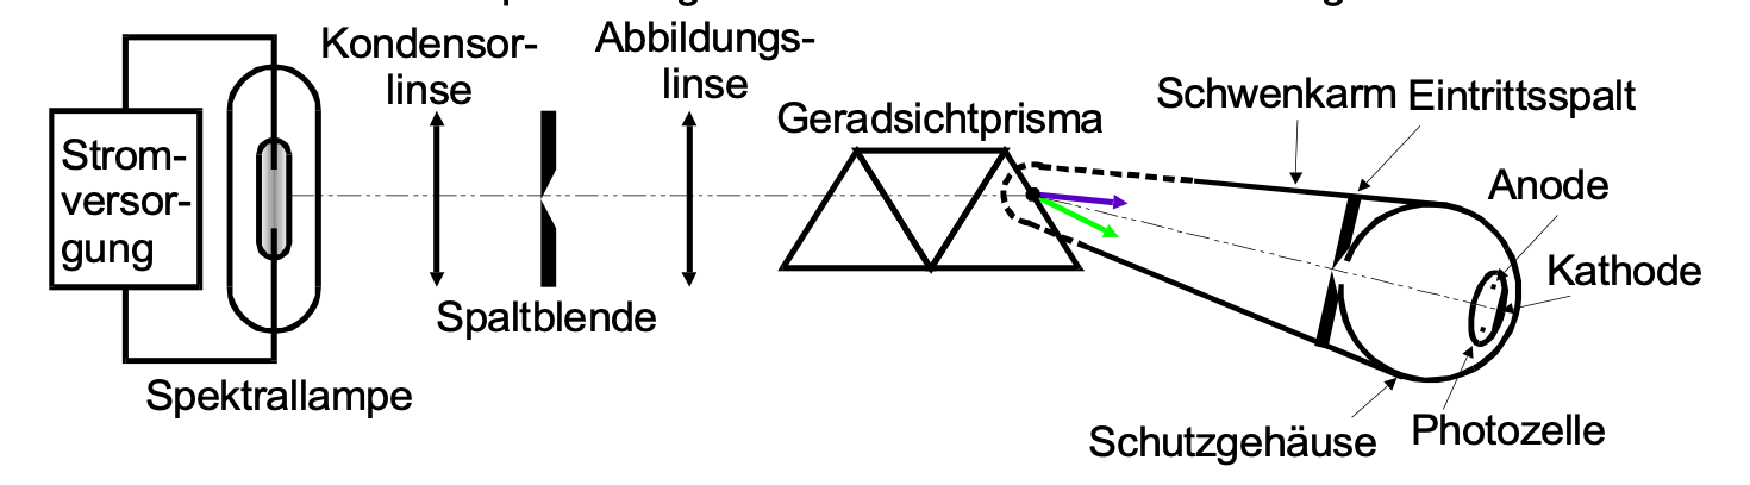
\includegraphics[height=4.5cm]{content/pics/Aufbau.pdf}
    \caption{Skizze des Aufbaus \cite{v500}.}
    \label{fig:Versuchsaufbau}
\end{figure}
Mithilfe zweier Linsen und einer Spaltblende wird das Licht der Quecksilberdampflampe auf ein Prisma fokussiert,
wo das Licht, aufgrund von Dispersion, wellenlängenabhängig gebrochen wird. In Folge dessen werden die 
Spektrallinien räumlich getrennt sichtbar.
Über einen Schwenkarm lässt sich die Photozelle so ausrichten, dass genau das Licht einer Spektrallinie durch
eine Spaltöffnung auf die Photokathode trifft.
Die Photozelle hat, wie in \autoref{fig:Photozelle_verwendet} zu sehen ist, eine ringförmige Anode, die 
in wenigen Millimetern Abstand parallel zu der Photokathode angeordnet ist.

\begin{figure}
    \centering
    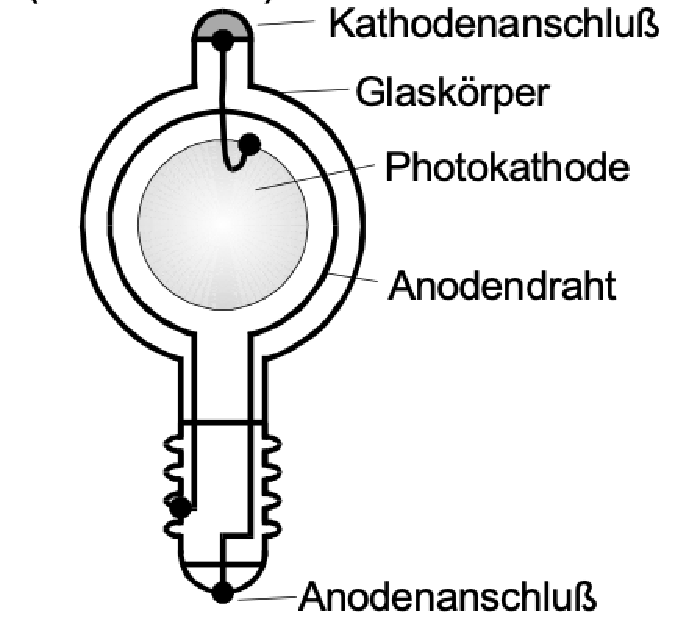
\includegraphics[height=6cm]{content/pics/Photozelle_verwendet.pdf}
    \caption{Skizze der verwendeten Photozelle \cite{v500}.}
    \label{fig:Photozelle_verwendet}
\end{figure}

Für die Messung des Photostroms und der Energie der Elektronen wird die Photokathode an eine regelbare
Spannungsversorgung angeschlossen. Außerdem wird ein Picoamperemeter verwendet, um den Photostrom zu messen.
Es ergibt sich ein Schaltbild wie in \autoref{fig:Schaltbild} zu sehen ist.

\begin{figure}
    \centering
    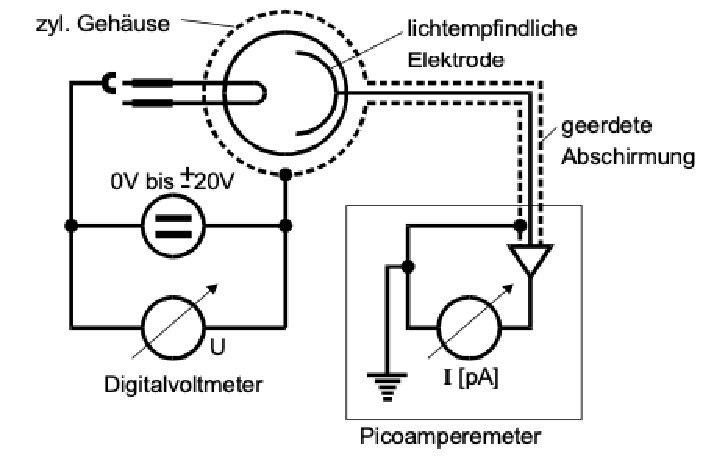
\includegraphics[height=6cm]{content/pics/Schaltbild.pdf}
    \caption{Elektrisches Schaltbild der Messapparatur \cite{v500}.}
    \label{fig:Schaltbild}
\end{figure}

\subsection{Messung des Photostroms}
Im Folgenden soll für 5 verschiedene Spektrallinien der Photostrom $I$ abhängig von der angelegten 
Bremsspannung $U_{\symup{B}}$ gemessen werden. Dafür wird die Spannung in angemessenen Schritten soweit
erhöht, bis der Photostrom zum erliegen kommt. Für die rote Spektrallinie wird nicht bei einer Bremsspannung
von $U_{\symup{B}} = \qty{0}{\volt}$ gestartet, sondern es wird eine Beschleunigungsspannung angelegt, damit
kein allzu kleiner Messbereich verwendet werden muss.

Außerdem wird für die gelbe Spektrallinie mit einer Wellenlänge von $\lambda=\qty{578}{\nano\metre}$ 
sowohl eine Beschleunigungsspannung, als auch eine Bremsspannung angelegt, sodass sich ein Messbereich
von $\qty{-20}{\volt} ≤ U_{\symup{B}} ≤ \qty{20}{\volt}$ ergibt.